%\documentclass[aps,twocolumn,secnumarabic,balancelastpage,amsmath,amssymb,nofootinbib, floatfix]{revtex4}
\documentclass[aps,twocolumn,secnumarabic,balancelastpage,amsmath,amssymb,nofootinbib,floatfix]{revtex4-1}
%\documentclass[5p]{elsarticle}
\newcommand{\abs}[1]{\lvert#1\rvert}

\usepackage{graphicx}      % tools for importing graphics
%\usepackage{lgrind}        % convert program code listings to a form 
                            % includable in a LaTeX document
%\usepackage{xcolor}        % produces boxes or entire pages with 
                            % colored backgrounds
%\usepackage{longtable}     % helps with long table options
%\usepackage{epsf}          % old package handles encapsulated postscript issues
\usepackage{bm}            % special bold-math package. usge: \bm{mathsymbol}
%\usepackage{asymptote}     % For typesetting of mathematical illustrations
%\usepackage{thumbpdf}
\usepackage{amsmath}
\usepackage{amssymb}
\usepackage{lipsum} 
\usepackage[colorlinks=true]{hyperref}  
\DeclareMathOperator\erfc{erfc}
\graphicspath{{../plots/}}

\begin{document}
\title{Measuring $^{nat}$La(p,x) Cross Sections from 35-60 MeV by Stacked Foil Activation}
\author{Jonathan T. Morrell}
%\email{jmorrell@berkeley.edu}
%\homepage{http://www.jonathanmorrell.info/} %If you don't have one, just comment out this line.
\date{\today}
%\affiliation{University of California, Berkeley - Nuclear Engineering}
\setlength{\parskip}{1em}

\begin{abstract}
In this experiment we use the stacked foil activation technique to measure cross sections for the $^{nat}$La(p,x) reaction, with proton energies in the 35-60 MeV range.  The primary motivation for this measurement is to quantify the production of $^{134}$Ce, a positron-emitting analogue of the medical isotope $^{225}$Ac, which has applications for kinetic bio-distribution assays of new radio-pharmaceuticals.  The results of this measurement show significant deviations from the cross sections modeled by the TALYS and EMPIRE nuclear reaction codes using default parameters.  There are no previous measurements of this reaction for comparison.
\end{abstract}

\maketitle


\section{Introduction}
Proton induced nuclear reactions in the tens of MeV range are used for the production of radioactive isotopes with minimal contaminants, making them a compelling production mechanism for diagnostic and therapeudic medical isotopes \cite{TARKANYI2016262}.  Nuclear data for many of these reactions is scarce, yet is critical for researchers wishing to optimize production schemes for these radioisotopes \cite{nuclear_data_needs}.

In this experiment, we measure the $^{nat}$La(p,x) reaction cross sections with a particular interest in the (p,6n) reaction on $^{139}$La (99.9119\% n.a.) for the production of $^{134}$Ce, a medically relevant isotope.  This experiment is also meaningful to the reaction modelling community, as this will be the first measurement of these cross sections.  These reactions are highly sensitive to pre-eqillibrium and nuclear spin-state distributions, and the results of this experiment will be useful for the comparison of various nuclear models. \cite{OTUKA2014272, PhysRev.87.366, nuclear_data_needs}.

\subsection{Motivation}
$^{225}$Ac is a promising candidate for new alpha-emitting radio-pharmaceuticals \cite{BOLL2005667}.  $^{225}$Ac has a half-life of 10 days, and decays to the stable $^{209}$Bi through the emission of 4 $\alpha$ and 2 $\beta^-$ particles. The longest half-life of any of the intermediates in the decay chain is the the 3.2 h $^{209}$Pb.  Also, many potential ligands are available for the chelation of $^{225}$Ac.  These properties make $^{225}$Ac a very compelling candidate for targeted radio-therapy \cite{BOLL2005667}.  However, before $^{225}$Ac can be tested on human subjects its performance must be quantified with biodistribution assays \cite{doi:10.1021/ac0580114}.  Unfortunately, the standard for these assays is to use positron emission tomography, which isn't possible with $^{225}$Ac because its decay chain doesn't include the emission of any positrons.

Instead, $^{134}$Ce has been proposed as a candidate isotope to be used as a positron emitting analogue of $^{225}$Ac, for use in rapid throughput kinetic biodistribution assays.  $^{134}$Ce decays with a half-life of 3.16 days, which is the closest of the $\beta^+$ emitting Ce isotopes to the 10 day half-life of $^{225}$Ac \cite{ensdf}.  It's daughter $^{134}$La also $\beta^+$ decays with a very short half-life (6.4 minutes), increasing its effectiveness as a biodistribution monitor.  

The proposed mechanism for the production of $^{134}$Ce is through the $^{139}$La(p,6n) reaction, using natural Lanthanum which has an isotopic abundance of $^{139}$La of 99.91 \%.  To date, this cross section has not been measured experimentally, and the predictions of the extensively used TALYS \cite{TALYS} and EMPIRE \cite{HERMAN20072655} nuclear reaction modelling codes differ by an order of magnitude (see figure \ref{fig:134CE}).  The objective of this experiment is to measure this cross section, as well as that of any other $^{nat}$La(p,x) reaction observable using the delayed-$\gamma$ stacked foil activation technique.


\section{Methodology}
In a stacked foil activation experiment one can measure a reaction cross section by measuring the activity induced within a thin foil of known areal number density, by a beam of known intensity \cite{GRAVES201644}.  Many such foils can be placed in a "stack", and the cross section can be measured at many different energies by a careful characterization of the energy loss within the stack.

The cross section for a given incident beam energy can be calculated using the activation method with the following equation:

\begin{equation}
\sigma =  A_0[I_p \rho \Delta r (1-e^{-\lambda t_i})]^{-1}
\label{eq:xs_calc}
\end{equation}

where $A_0$ is the activity of a given reaction product at the end of irradiation, $I_p$ is the proton beam current, $\rho \Delta r$ is the areal number density. The factor $(1-e^{-\lambda t_i})$ is the ratio of induced activity to the saturation activity assuming single-step production and decay, where $\lambda$ is the decay constant for a given reaction product and $t_i$ is the total irradiation time.  

In this experiment the areal number density was determined by measuring the mass $m$, the area $A$ and the thickness $\Delta r$, and was calculated according to the equation

\begin{equation}
\rho \Delta r=\frac{w\cdot m \cdot N_A}{MA\Delta r}\Delta r = \frac{w\cdot m \cdot N_A}{MA}
\label{eq:number_density}
\end{equation}
where $w$ is the isotopic abundance in the sample, $M$ is the molar mass and $N_A$ is Avagadro's number.  

Following irradiation, the delayed $\gamma$-rays emitted by the proton induced reaction products were counted using a high-purity germanium (HPGe) detector to determine the end-of-beam activity $A_0$ of a given reaction product.  If a $\gamma$ spectrum is counted for a measurement time $t_m$, beginning some amount of time $t_c$ after the beam is shut off, then the end-of-beam activity measured in a photo-peak having $N_c$ counts is given by

\begin{equation}
A_0 = \frac{\lambda N_c}{(1-e^{-\lambda t_m})e^{-\lambda t_c}I_{\gamma}\epsilon}
\label{eq:activity}
\end{equation}

where $I_{\gamma}$ is the $\gamma$ emission fraction per decay and $\epsilon$ is the detector efficiency at the energy of the photo-peak.

The proton beam current $I_p$ was determined using a copper and aluminum monitor foil for each lanthanum foil in the stack.  These foils have multiple reaction channels with very well characterized cross sections \cite{IAEACPR}, allowing for precise determination of the beam current using a very similar activation procedure to that described by equation \ref{eq:xs_calc}, where instead of calculating the cross section using a known beam current we calculate the beam current using a known cross section, i.e.

\begin{equation}
I_p =  A_0[\sigma \rho \Delta r (1-e^{-\lambda t_i})]^{-1}
\label{eq:beam_current}
\end{equation}

Because the proton beam isn't characterized by a single energy, but rather an energy spectrum $\psi(E)$, the cross-section used in the beam current calculation should be replaced by an average cross-section $\bar{\sigma}$ given by

\begin{equation}
\bar{\sigma} = \frac{\int_0^{\infty}\sigma\psi(E)dE}{\int_0^{\infty}\psi(E)dE}
\label{eq:avg_xs}
\end{equation}

This energy spectrum was determined for each foil in the stack using a Monte Carlo implementation of the Anderson-Ziegler stopping power tables \cite{ZIEGLER20101818}.



\subsection{Description of Experiment}

The lanthanum foils used in this experiment were cold rolled to 25 $\mu$m thickness, cut to 1" by 1" squares, and sealed in glass ampules with an inert cover gas (to prevent oxidation).  Just prior to the experiment these ampules were opened, their dimensions and masses were measured, and they were then sealed in kapton tape.  The copper and aluminum monitor foils were cut from 25 $\mu$m thick sheets into 1" by 1" squares, and were also measured and sealed in kapton tape.  These foil packets were then secured onto 2.25" by 2.25" aluminum sample holders (see Fig. \ref{fig:expt_photos}), which served to both protect the foils during handling and center them in the beam.  10 sets of aluminum, copper and lanthanum foil packets were prepared in this manner for cross section measurements at 10 energies.

\begin{figure}[htb]
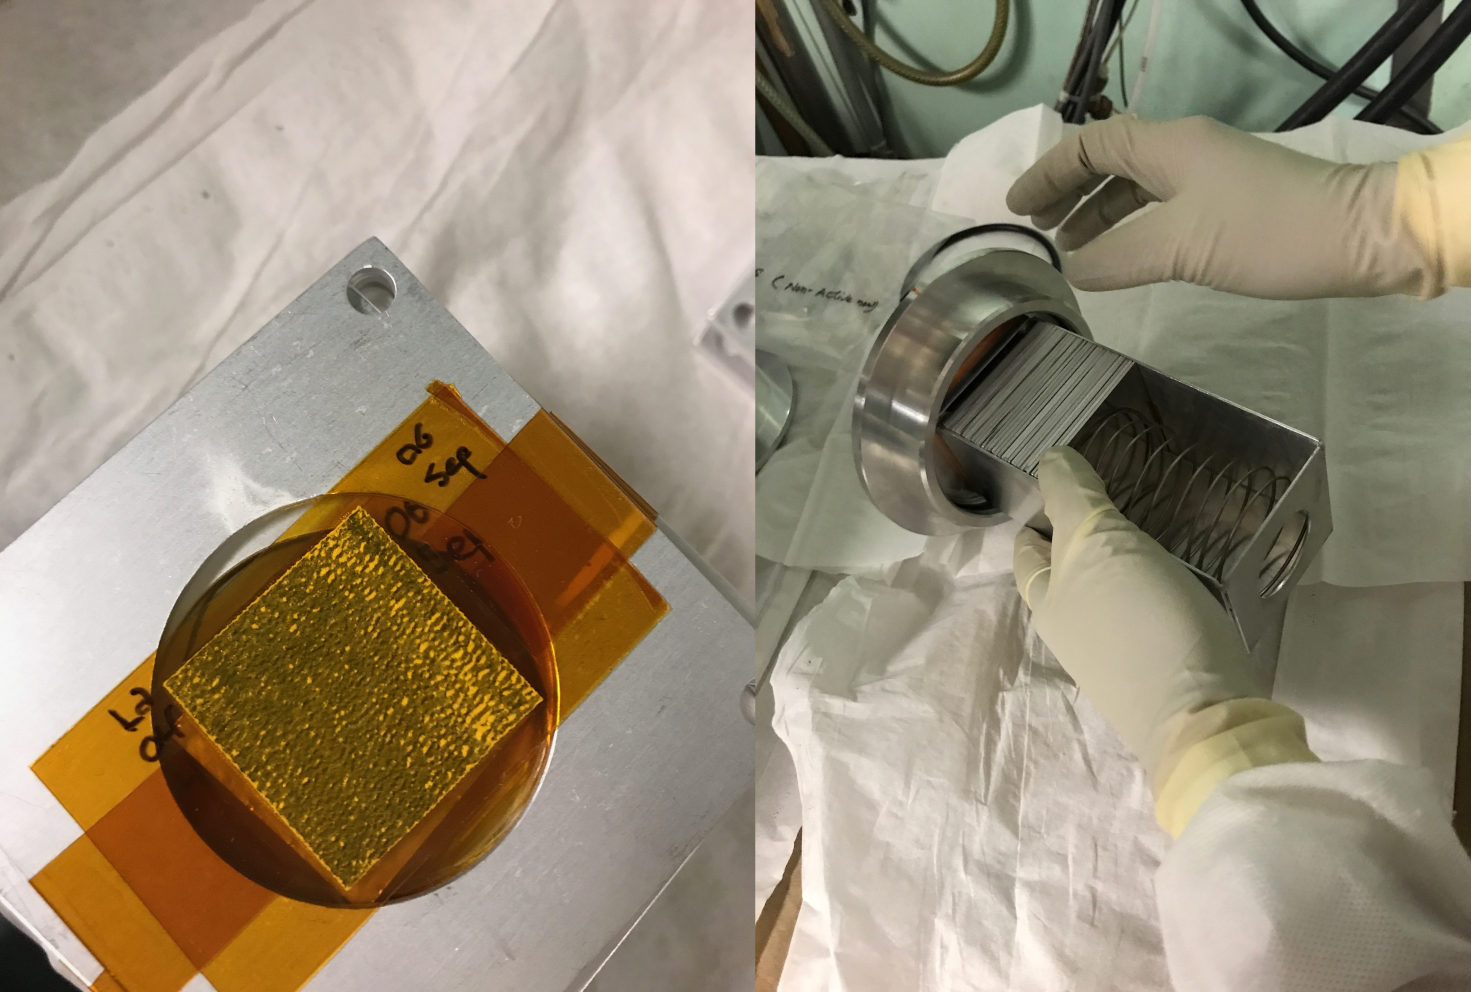
\includegraphics[width=9cm]{photos/foil_stack.png}
\caption{Photo of an individual foil packet secured to the aluminum sample holder (left) and the entire foil stack (right).  The front of the stack (facing the beam) is oriented towards the right in this photo.   
}
\label{fig:expt_photos}
\end{figure}

Multiple thick aluminum plates, also 2.25" by 2.25", were placed in between each set of foil packets to degrade the beam energy by a few MeV (per degrader), covering the proton energy range from 35 - 60 MeV.  The appropriate thickness for each aluminum degrader was selected using an Anderson \& Ziegler calculation, however the actual proton energy distributions seen by each foil were determined using the monitor foils themselves.  This is described in more detail in section \ref{monitors}.

Additionally, stainless steel foils were placed at the front and back of the stack.  Post-irradiation dose mapping using radio-chromic films confirmed that the proton beam was centered on the samples, and that the entirety of the beam was contained well within the 1" by 1" borders of the foil packets.

\subsection{Facility Overview}
This experiment took place using a 60 MeV proton beam at the 88" cyclotron located at Lawrence Berkeley National Lab in Berkeley, California USA.  The 88" cyclotron is a K=140 sector focused cyclotron with a maximum proton energy of 60 MeV and a maximum proton beam current of approximately 20 $\mu$A.

The 88" cyclotron facility has several isolated beamlines for a multitude of applications (see Fig. \ref{fig:cyclotron}).  This experiment took place in Cave 0, which has a ~3m beam pipe which is shielded from the radiation produced in the cyclotron vault.  The foil stack was located at the end of this beam pipe, which is downstream from two bending magnets and several focusing quadrupoles, ensuring that the beam was well collimated and mono-energetic.

\begin{figure}[htb]
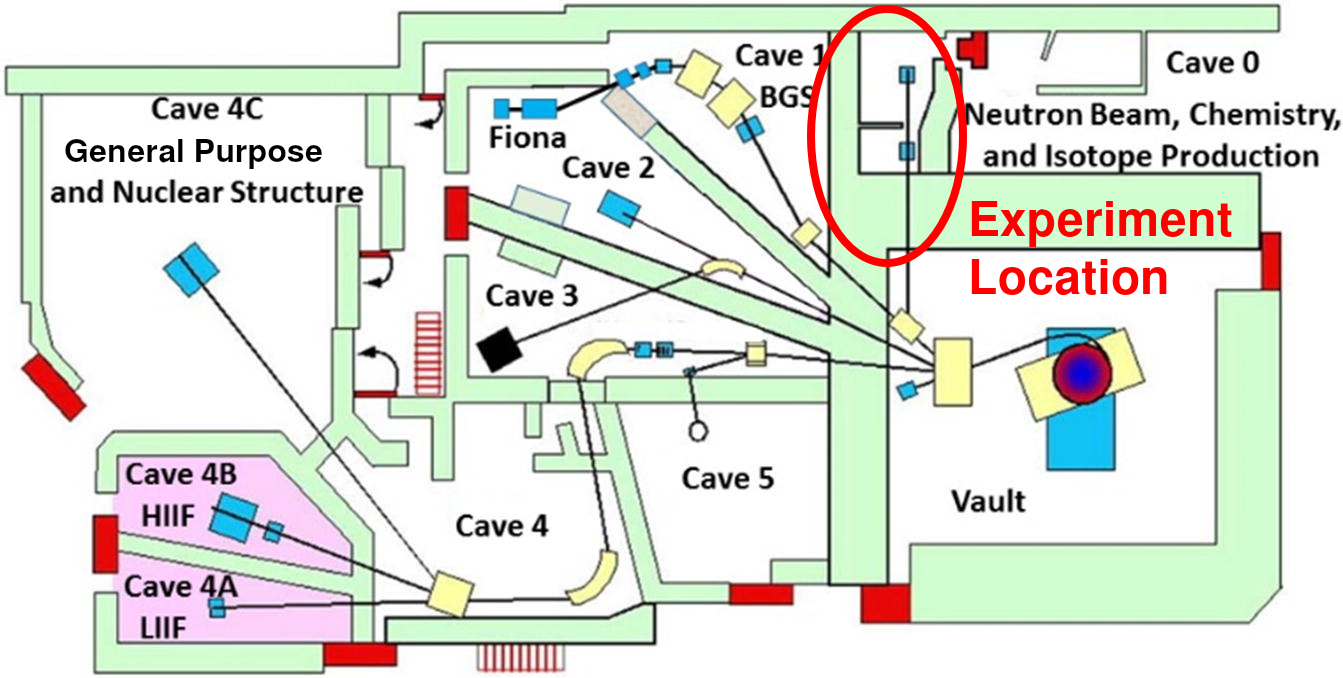
\includegraphics[width=9cm]{photos/cyclotron.png}
\caption{Graphical representation of the 88" cyclotron floor plan.  The irradiation performed in this experiment took place in Cave 0.
}
\label{fig:cyclotron}
\end{figure}

This experiment marks the first time the 88" cyclotron has attempted operating with 60 MeV protons.  The cyclotron and beam transport elements were operating at their extreme limits, which meant the peak transmission out of the cyclotron and to the sample holder was about 8 nA.  The stack was irradiated for 1 hour and 37 minutes, which yielded enough activity to measure all cross sections of interest to approximately 5\% uncertainties.


\subsection{Detector Calibration}

The energy and efficiency of the HPGe detector used in this measurement were calibrated using 4 standard calibration sources of known activity (rel. error $<$1\%): $^{137}$Cs, $^{152}$Eu, $^{54}$Mn and $^{133}$Ba.

A linear calibration of the $\gamma$-ray energy $E$ to the MCA channel number $N$, $E = m\cdot N+b$, was applied, and a plot of the residuals (Fig. \ref{fig:energy_calibration}) shows that this is the correct functional form of the energy calibration, i.e. that there is no quadratic component to the detector response.

\begin{figure}[htb]
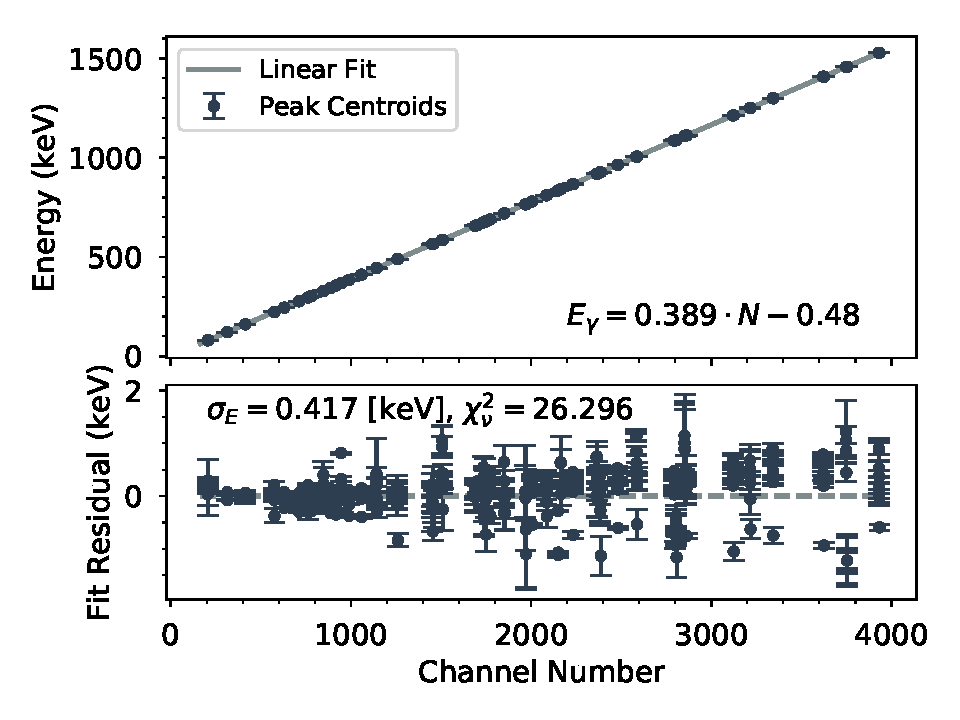
\includegraphics[width=9cm]{calibration/energy_calibration.pdf}
\caption{Linear energy calibration, and plot of the fit residuals.
}
\label{fig:energy_calibration}
\end{figure}

A modified 2$^{nd}$ order polynomial was applied for the detector efficiency calibration, using the equation

\begin{equation}
\epsilon (E) = exp[a\cdot ln(E)^2+b\cdot ln(E)+c]
\end{equation}

where $\epsilon$ is the efficiency and $a$, $b$, and $c$ are fitting coefficients.  The efficiency was measured at multiple distances from the detector, ranging from 1 cm to 60 cm.  The resulting fits for the detector efficiency used in this experiment are plotted in figure \ref{fig:efficiency_calibration}, showing reasonably good agreement.

\begin{figure}[htb]
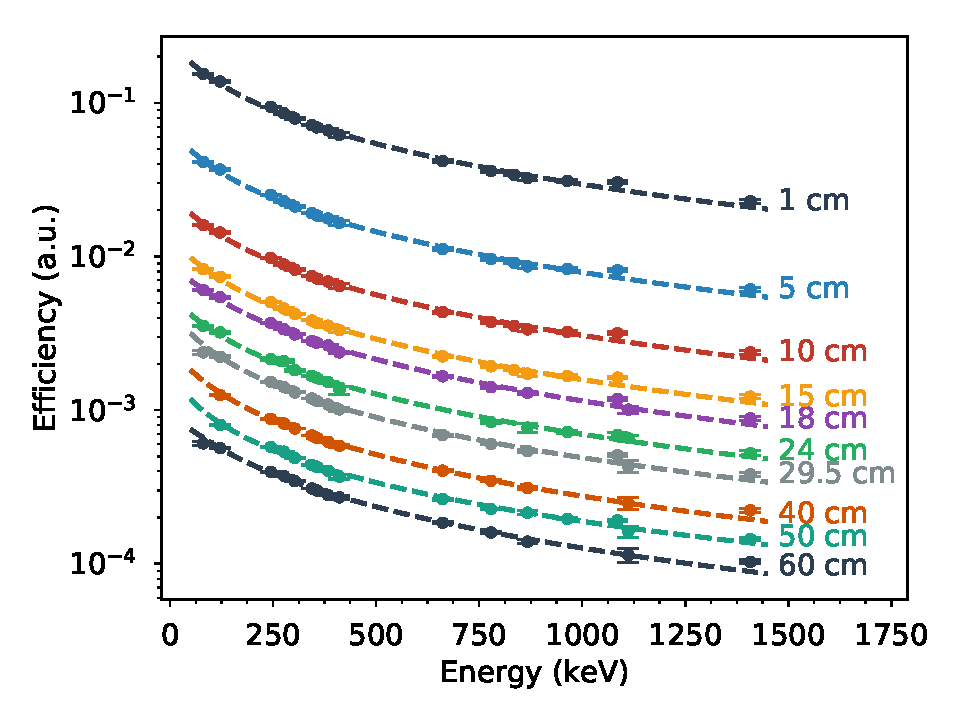
\includegraphics[width=9cm]{calibration/efficiency_calibration.pdf}
\caption{Detector efficiency calibration, relative to $\gamma$ emitting efficiency standard of known activity.
}
\label{fig:efficiency_calibration}
\end{figure}

\subsection{Irradiation and Counting}
The foils were irradiated with 8 nA of proton current for 1 hour, 37 minutes and 24 seconds.  The total collected charge of the beam was measured using a current integrator at the beam dump, which was only used as a rough approximation of the beam current to compare with the values measured by the monitor foils.

After irradiation, the foils were removed from the beamline and transferred to the HPGe counting lab.  Upon removal it was discovered that the third lanthanum foil showed excessive oxidation (prior to counting), therefore the cross sections from this foil had to be discarded.

The subsequent foil counting took place over the next 4 weeks.  Each foil was counted multiple times, in order to reduce uncertainty and aid in isotope identification.  The lengthy counting duration was necessary because the 604.6 and the 606.8 keV lines from the $^{135}$Ce isotope significantly contaminated the 604.7 keV line in the $^{134}$Ce daughter isotope $^{134}$La. Because the $^{134}$Ce isotope has a longer half life, it was able to be accurately counted after the $^{135}$Ce isotope had decayed to negligible levels.

\section{Data Analysis}
The general procedure for calculating cross sections proceeds as follows.  First, every $\gamma$ line emitted from each isotope of interest was fit in each spectrum collected.  The number of counts in each peak was used to determine the activity of the isotope at the time the spectrum was taken, and these activities as a function of "cooling" time was used to calculate the activity of that isotope at the end of irradiation.  This activity $A_0$ was then used to calculate a cross section (for the lanthanum foil data) or a beam current (for the copper/aluminum foil data).  The energy assignments for each foil was determined using a variation of parameters approach, discussed in section \ref{monitors}.

\subsection{Peak Fitting}

\begin{figure}[htb]
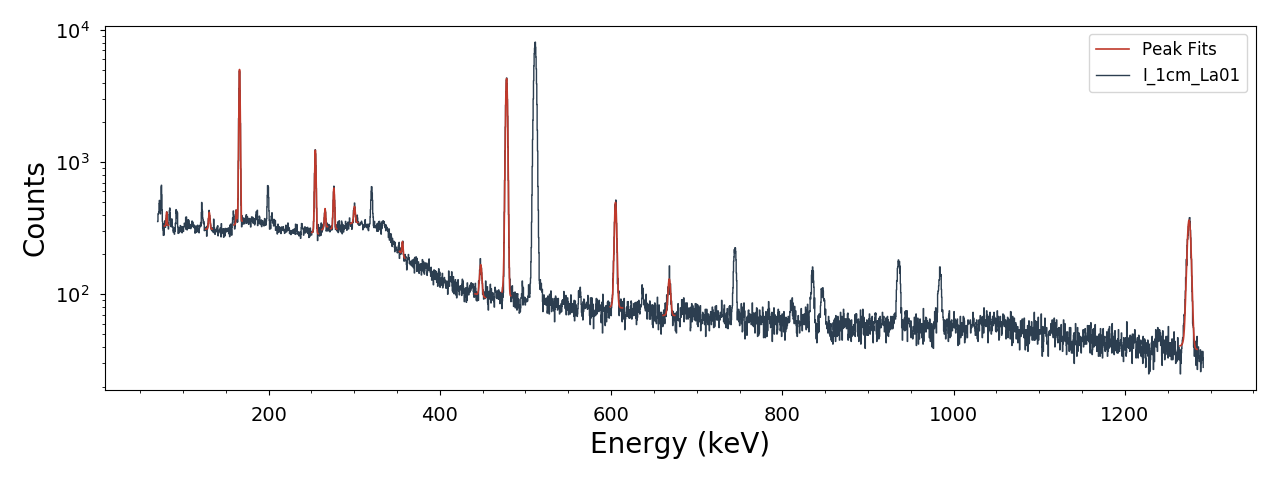
\includegraphics[width=9cm]{peak_fits/I_1cm_La01_fits}
\caption{Example of $\gamma$-ray spectrum from the first lanthanum foil, with peak fits indicated in red.
}
\label{fig:peak_fit}
\end{figure}

The detector energy and efficiency calibration, as well as the induced activity in each sample, was ultimately determined by peak fitting to the individual spectra.  Energy centroids and relative intensities were constrained with some uncertainty by the decay data given by the National Nuclear Data Center (NNDC) \cite{ensdf}, also listed in Appendix \ref{nudat_appendix}.  Where uncertainties were not listed, they were assumed to be 10 \%.  Each peak was fit with a skewed Gaussian function on top of a linear background. Knoll recommends this as the functional form of a photopeak in an HPGe spectrum because localized charge trapping in the Ge crystal will lead to "tailing" on the low-energy side of the peak \cite{Knoll}.  The complete functional form of the peak fit, $F(i)$, as a function of channel number $i$ is as follows.

The "background" under each photopeak, which could be due to actual background radiation or Compton scattering, was given a linear form:

\begin{equation}
F_{bg}(i) = m\cdot i + b
\label{eq:background}
\end{equation}

This is purely heuristic but is accurate in most cases because the background tends to be slowly varying over the energy range of one photopeak \cite{gammas}.  The resolution function for HPGe detectors is Gaussian, which means that the convolution of a photopeak (which can be assumed to be a delta function) with the resolution function simply gives a Gaussian peak shape:

\begin{equation}
F_{gauss}(i) = A\cdot \exp (-\frac{(i-\mu)^2}{2\sigma^2})
\label{eq:gaussian}
\end{equation}

where $A$ is the height of the peak, $\mu$ is the mean or centroid and $\sigma$ is the standard deviation, sometimes called the width of the peak.

The low energy tailing in an ideal detector is characterized by an exponential with argument $\frac{i-\mu}{\beta}$, where $\beta$ is a width parameter.  Convolution of this exponential with a Gaussian resolution function gives a skewed Gaussian:

\begin{equation}
F_{skew}(i) = B\cdot \exp (\frac{i-\mu}{\beta}) \erfc (\frac{i-\mu}{\sqrt{2}\sigma}+\frac{\sigma}{\sqrt{2}\beta})
\label{eq:skew}
\end{equation}

where $B$ is the height of the skewed Gaussian.  In general, $B$ is prortional to $A$, and $\beta$ is proportional to $\sigma$.  We will take advantage of this fact to better constrain our peak fits, as the number of parameters is already somewhat large.  Re-configuring the parameters $B$ and $\beta$ as $B = R\cdot A$, $\beta = \alpha \cdot \sigma$ means the parameters characterizing the skewed Gaussian will only have small variations between peaks and can be fit with much tighter bounds.  For this experiment these skewed Gaussians were found to be approximately parameterized by $R \approx 0.2$ and $\alpha \approx 0.9$.

Finally, the complete equation for individual photopeaks is given by:

\begin{align*}
F_{peak}(i) &= m\cdot i + b + A\cdot [\exp (-\frac{(i-\mu)^2}{2\sigma^2}) \\
& + R\cdot \exp (\frac{i-\mu}{\alpha \sigma}) \erfc (\frac{i-\mu}{\sqrt{2}\sigma}+\frac{1}{\sqrt{2}\alpha})]
\label{eq:peak}
\end{align*}


An example of a measured $\gamma$-ray spectrum is shown if Fig. \ref{fig:peak_fit}, with photo-peak fits superimposed on the spectrum.

\subsection{Determining Foil Activities}
\label{eob_activities}

For a single photopeak having $N_c$ counts observed with efficiency $\epsilon$ from a radioactive nucleus with decay constant $\lambda$ and intensity $I_{\gamma}$, equation \ref{eq:activity} can be used to calculate the end-of-beam activity for a given isotope.  However, if multiple photopeaks are to be used in the calculation, the activity in a photopeak at some cooling time $t_c$ after the end-of-beam can be calculated by

\begin{equation}
A(t_c) = \frac{\lambda N_c}{(1-e^{-\lambda t_m})I_{\gamma}\epsilon}
\end{equation}

where $t_m$ is the measurement time.  The end-of-beam activity $A_0$ can then be calculated by a Levenberg Marquardt fit to the equation

\begin{equation}
A(t_c) = A_0e^{-\lambda t_c}
\label{eq:decay}
\end{equation}

This method is much more robust to outliers, and will significantly reduce the uncertainty in the initial activity $A_0$.  An example of a fit to this exponential decay curve is shown in Fig. \ref{fig:decay_curves}.

\begin{figure}[htb]
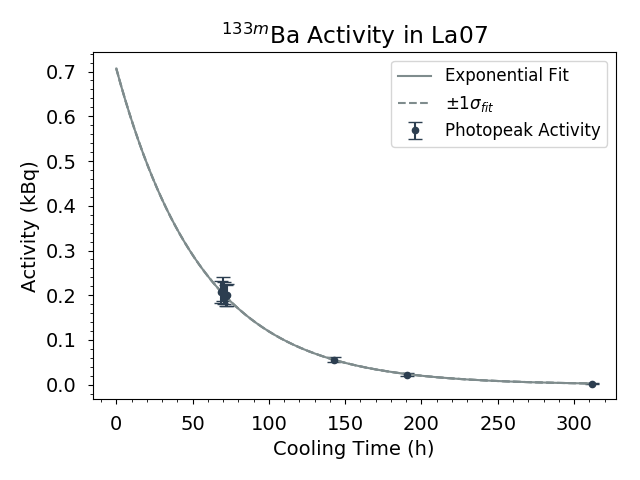
\includegraphics[width=9cm]{decay_curves/La07_133BAm}
\caption{Example of a decay curve and assosiated exponential fit used to calculate the initial activity of the $^{133m}$Ba isotope in the 7$^{th}$ lanthanum foil.  The uncertainty in the fit is very small ($<$1\%). The dominant contribution to the systematic uncertainty in $A_0$ was the evaluated half-life for most of the observed reactions.
}
\label{fig:decay_curves}
\end{figure}

However not all of the isotopes measured in this experiment follow the simple one-step decay pathway.  $^{134}$Ce for example, decays to $^{134}$La which then decays to $^{134}$Ba, which is stable.  For these two-step decay chains, the decay curve will be of the shape

\begin{equation}
A_D(t_c) = A_{p0}\frac{\lambda_D}{\lambda_D - \lambda_p}(e^{-\lambda_p t_c}-e^{-\lambda_D t_c})+A_{D0}e^{-\lambda_D t_c}
\end{equation}

where the subscript $p$ indicates the parent isotope and $D$ the daughter.  This required an estimation of the initial parent activity $A_{p0}$ using a fit to equation \ref{eq:decay}, which somewhat increased the uncertainty in the calculation of the initial daughter activities.

\subsection{Current Monitors and Energy Assignments}
\label{monitors}

The proton beam current on each foil for a given monitor reaction channel can be calculated according to equation \ref{eq:beam_current}, where the activity $A_0$ is determined from the decay curves as previously described.  Measured currents for the three copper monitor reactions and the two aluminum reactions are plotted in Fig. \ref{fig:beam_current}, as well as a linear fit to these values. This fit was used to interpolate the beam current witnessed by the lanthanum foils.  As the beam didn't react greatly in the thin foils, the current was roughly constant through the stack. There was no underlying assumption justifying a linear fit, it simply gave the best reduced $\chi^2$ for the interpolation.

\begin{figure}[htb]
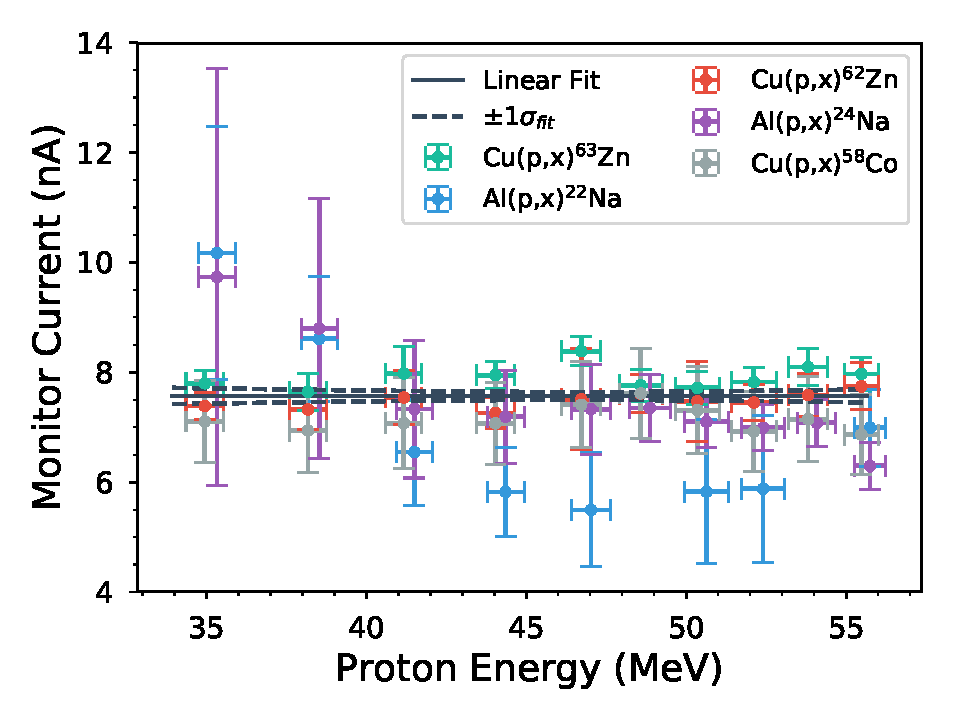
\includegraphics[width=9cm]{monitors/current_norm_mcnp}
\caption{Plot of the proton beam current measured by each of the monitor foil reaction channels, with a linear fit that was used to calculate the current for the lanthanum foils.
}
\label{fig:beam_current}
\end{figure}

As can be seen in the plot the uncertainty in both aluminum monitor reactions was rather large, particularly in the $^{27}$Al(p,$\alpha$pn)$^{22}$Na reaction.  This was due to contaminating reactions in the Kapton tape that sealed the foils, $^{28}$Si(p,$\alpha$2pn)$^{22}$Na and $^{28}$Si(p,4pn)$^{24}$Na, which had to be corrected for.  This correction was performed by measuring the activities of the $^{22}$Na and $^{24}$Na isotopes in the Kapton sealing the neighboring lanthanum and copper foils, and subtracting this contribution from the aluminum foil data.

Secondary neutron production could have also contributed to $^{22,24}$Na activation, however the measured activities weren't consistent with neutron activation. Also, the secondary neutron flux predicted by our MCNP model was 3-4 orders of magnitude lower than the proton flux, so we don't have reason to believe it affected the measured beam currents \cite{MCNP}.

As mentioned previously, the beam currents measured in each monitor foil reaction channel were were determined using the flux-averaged cross sections, given by equation \ref{eq:avg_xs}.  This accounted for the fact that the beam had significant energy spread, particularly toward the back of the stack, and the reaction cross-sections were often not smoothly varying.  $\psi(E)$ was determined using an Anderson-Ziegler model \cite{ZIEGLER20101818}.  A plot showing the flux spectra for each foil in the stack, as predicted by Anderson-Ziegler, is shown in figure \ref{fig:az_spectrum}.

\begin{figure}[htb]
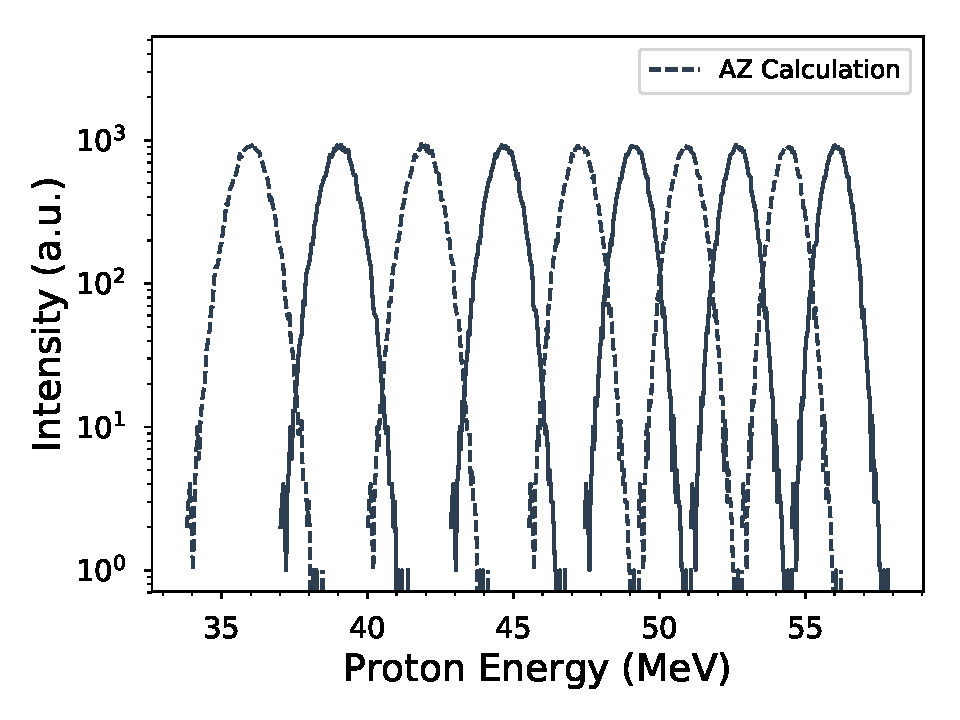
\includegraphics[width=9cm]{monitors/La_az_spectrum}
\caption{Plot of the proton energy spectra for each lanthanum foil in the target stack.  Dashed lines are only to provide visual clarity.
}
\label{fig:az_spectrum}
\end{figure}

\subsection{Optimization of Energy Assignments}

The energy centroids and 1 $\sigma$ values were first estimated using the Anderson-Ziegler output, however there was a large spread in the apparent beam current values seen by each monitor reaction channel.  This spread was particularly high for the foils on the low energy side of the stack, which was where the monitor cross sections varied the most.  This was indicative of incorrect characterization of the proton energy spectra incident on each monitor foil.

In order to correct for this effect, the effective areal density of the degrader foils and the incident proton beam energy were treated as free parameters, and were varied in order to find the energy assignments yielding the smallest variance in the beam current \cite{GRAVES201644}.

It's important to note that this treatment doesn't imply that the degrader density was actually less or greater than was measured, rather that there was some energy loss taking place that wasn't accounted for in the original model.  In essence, we are assigning energy spectra to each foil that will make the shape of the measured monitor reaction cross sections match the shape of the known charged-particle reference standards.

\begin{figure}[htb]
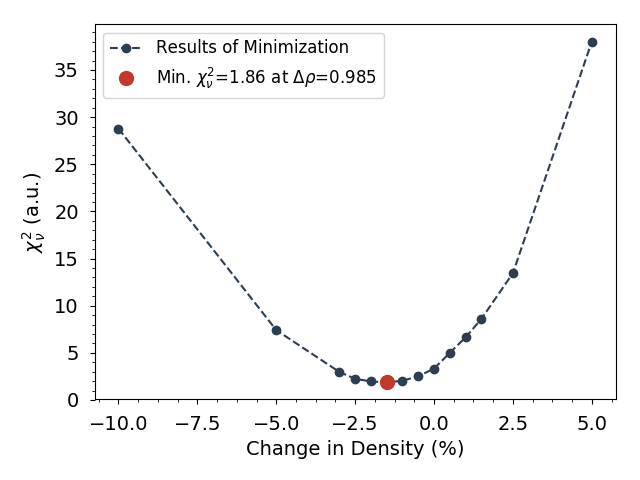
\includegraphics[width=9cm]{monitors/minimize_az}
\caption{Plot of the reduced $\chi^2$ for the current monitor data, as the effective density of the degraders was varied.
}
\label{fig:minimization}
\end{figure}

Figure \ref{fig:minimization} shows the results of the minimization at an incident proton energy of 57 MeV.  The reduced $\chi^2$ of the linear fit to the monitor foil currents (shown in Fig \ref{fig:beam_current}) was used to determine the optimum energy assignments, given by the Anderson-Ziegler model with varied degrader foil densities.  $\chi^2_{\nu}$ was preferred over other figures of merit because the aluminum monitor channels had large uncertainties, and would have otherwise overly contributed to the resulting energy assignments.

The results of this minimization show that the optimum energy assignments correspond to no change in the effective areal density of the stack, however they do show that the incident proton beam energy was 57 MeV, rather than the expected 60 MeV.  This was a surprisingly large deviation from the initial estimates.  The incident proton beam energy could have been affected by a number of experimental factors.  This was the highest energy proton beam to date at the LBNL 88" cyclotron, and the main magnetic field may be less well characterized for this tune.  Also, the transmission out of the cyclotron was very poor, about 0.1\%.  It could be that the portion of the beam that was extracted wasn't at the expected energy, and that the deflector fields weren't set high enough to extract the 60 MeV portion of the beam.

%As for the 15\% deviation from the expected areal density, this could be attributed to a measurement error (of the foil densities), or a modelling error.  Interestingly, an Anderson and Ziegler (SRIM/TRIM) calculation gave optimum energy assignments for 0\% deviation, which means that something may have been wrong with either the MCNP input, or the data it uses.

The minimization was also performed with the Monte Carlo code MCNP \cite{MCNP}.  This yielded the same energy assignments, however the optimum change in areal density predicted by the MCNP model was 15\%, which suggests an error in either the MCNP input, or the stopping power tables used by MCNP.

\section{Results and Discussion}

Using the end-of-beam activities, beam currents, and energy assignments determined in the previous section, the cross sections were calculated according to equation \ref{eq:xs_calc}.  These measured results were compared to predictions from the TALYS and EMPIRE nuclear reaction codes using default parameters.  The pre-equillibrium model used in the EMPIRE calculations was the Hybrid Monte-Carlo Simulation module (HMS), while the TALYS code uses the exciton pre-equillibrium model \cite{HERMAN20072655, TALYS}. The results of these cross section measurements are described in more detail below, and the measured values are tabulated in Appendix \ref{xs_appendix}.

\subsection{$^{nat}$La(p,6n)$^{134}$Ce Cross Section}

$^{134}$Ce decays to $^{134}$La via a 98.9\% ground state to ground state electron capture, and there are consequently very few $\gamma$ emissions with which to measure a cross section.  The most intense is the 0.209\%, 130.4 keV $\gamma$-line \cite{ensdf}.  Instead of measuring a decay gamma from $^{134}$Ce, the 604.721 keV ($I_{\gamma}$=5.04 \%) line in the decay of the daughter isotope $^{134}$La was used to measure the $^{nat}$La(p,6n)$^{134}$Ce cross section.  This was possible because $^{134}$La decays with a 6.45 minute half-life, which meant that regardless of the initial population of $^{134}$La, all 604.7 keV $\gamma$'s emitted after several hours of decay time were attributable only to the initial $^{134}$Ce population.

Additionaly, $^{135}$Ce produces multiple decay $\gamma$'s very close in energy to the 604.7 keV line, which meant that roughly 2 weeks of post-irradiation cool down were required to make this cross section measurement without the $^{135}$Ce contaminant.

\begin{figure}[htb]
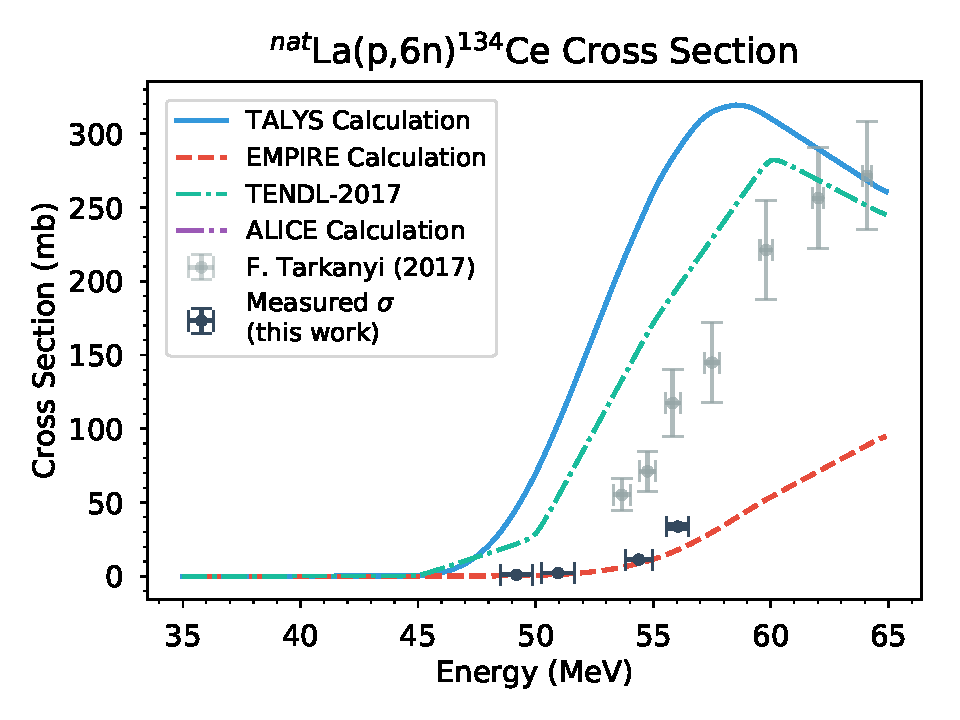
\includegraphics[width=9cm]{cross_sections/134CE}
\caption{Measured cross section for the $^{nat}$La(p,6n)$^{134}$Ce reaction, with TALYS (solid blue) and EMPIRE (dashed red) predictions.  Note that the TALYS calculation has been divided by 10.
}
\label{fig:134CE}
\end{figure}

The measured cross sections are plotted in Fig. \ref{fig:134CE}, along with the outputs of the TALYS and EMPIRE nuclear reaction codes using default settings.  Clearly the hybrid Monte Carlo simulation (HMS) pre-equillibrium model used by EMPIRE gives much better agreement with measured data than the exciton model used by TALYS.  This was not the case for all the measured reaction channels, and this dispersion is likely attributable to the fact that this reaction has not been measured in the pre-equillibrium energy range prior to this work, and so default parameters shouldn't be expected to give reliable results without some adjustment.

\subsection{$^{nat}$La(p,5n)$^{135}$Ce Cross Section}

The $^{nat}$La(p,5n)$^{135}$Ce reaction was perhaps the most amenable of those measured to the stacked foil activation technique, due to a high number of intense $\gamma$ emissions (e.g. 41.8\% for the 265.56 keV line) and 17.7 hour half-life.  As such these emissions tended to dominate most of the $\gamma$ spectra taken earlier in time, giving good statistics on this cross section.  Unfortunately, the 20 second isomer was too weak to measure by the time the foils had been transferred to the counting lab, so the reported cross sections are cumulative.  The uncertainties were on the order of 6\%, of which roughly 3\% came from the $I_{\gamma}$'s given by NUDAT and 1\% from the half-life.  

\begin{figure}[htb]
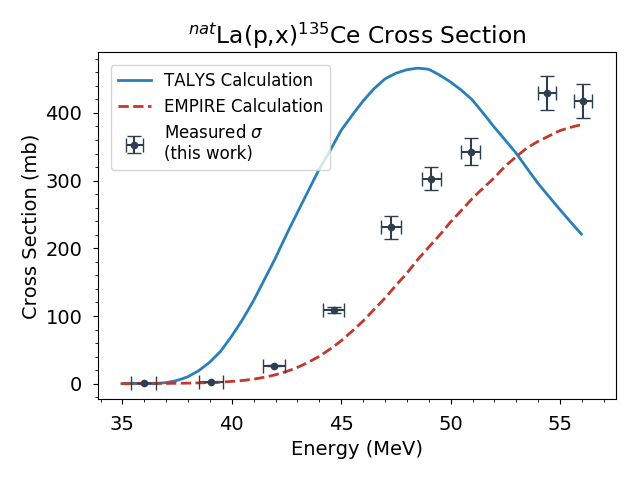
\includegraphics[width=9cm]{cross_sections/135CE}
\caption{Measured cross section for the $^{nat}$La(p,5n)$^{135}$Ce reaction, with TALYS (solid blue) and EMPIRE (dashed red) predictions.
}
\label{fig:135CE}
\end{figure}

The measured cross sections are plotted in Fig. \ref{fig:135CE}, along with the outputs of the TALYS and EMPIRE nuclear reaction codes using default settings.  While both codes approximately predicted the magnitude of this cross section, the energy at which it peaks is clearly mis-calculated by the TALYS exiton model.

\subsection{$^{nat}$La(p,3n)$^{137m,137g}$Ce Cross Sections}

The decays of both the 34.4 hour isomer and the 9.0 hour ground state in $^{137}$Ce were observable using delayed $\gamma$ spectroscopy, which allows for the measurement of the independent cross sections (i.e. the isomer to ground state ratio) for this reaction.  

\begin{figure}[htb]
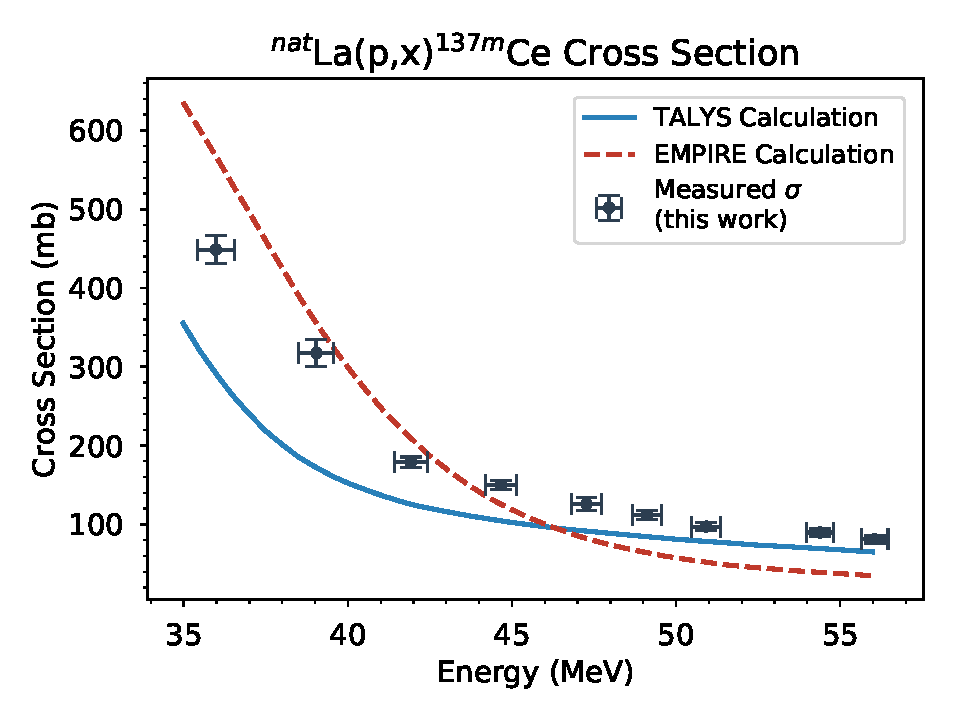
\includegraphics[width=9cm]{cross_sections/137CEm}
\caption{Measured cross section for the $^{nat}$La(p,3n)$^{137m}$Ce reaction, with TALYS (solid blue) and EMPIRE (dashed red) predictions.
}
\label{fig:137CEm}
\end{figure}

The measured cross sections for the $^{nat}$La(p,3n)$^{137m}$Ce reaction are plotted in Fig. \ref{fig:137CEm}, as well as the TALYS and EMPIRE default outputs.  The $^{nat}$La(p,3n)$^{137g}$Ce cross sections are plotted in Fig. \ref{fig:137CEg}.  In neither case is there a clear "best fit" in the models.  Both agree much better than in the (p,5n) or (p,6n) reactions, and likely an adjustment of the level density model or spin-cutoff parameters would bring the calculations into agreement with the data.

\begin{figure}[htb]
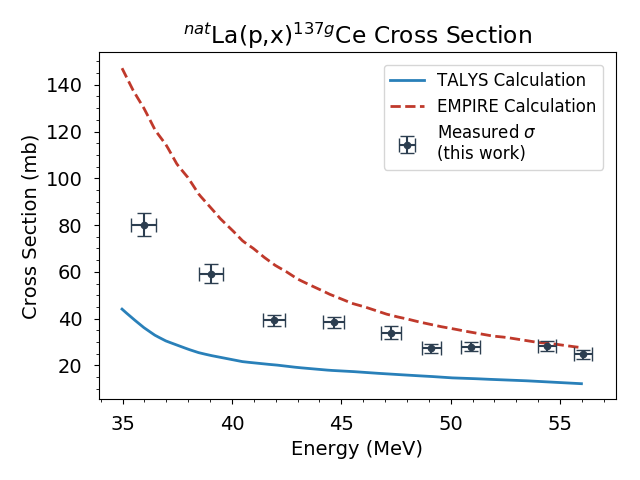
\includegraphics[width=9cm]{cross_sections/137CEg}
\caption{Measured cross section for the $^{nat}$La(p,3n)$^{137g}$Ce reaction, with TALYS (solid blue) and EMPIRE (dashed red) predictions.
}
\label{fig:137CEg}
\end{figure}

\subsection{$^{nat}$La(p,n)$^{139}$Ce Cross Section}

Measurement of the direct reaction was possible using the 80 \%, 165.85 keV $\gamma$ emission from the $^{139}$Ce ground state decay.  This was a cumulative cross section measurement, as the 58 second isomer decayed to a negligible activity before it was able to be counted with the HPGe detector.

\begin{figure}[htb]
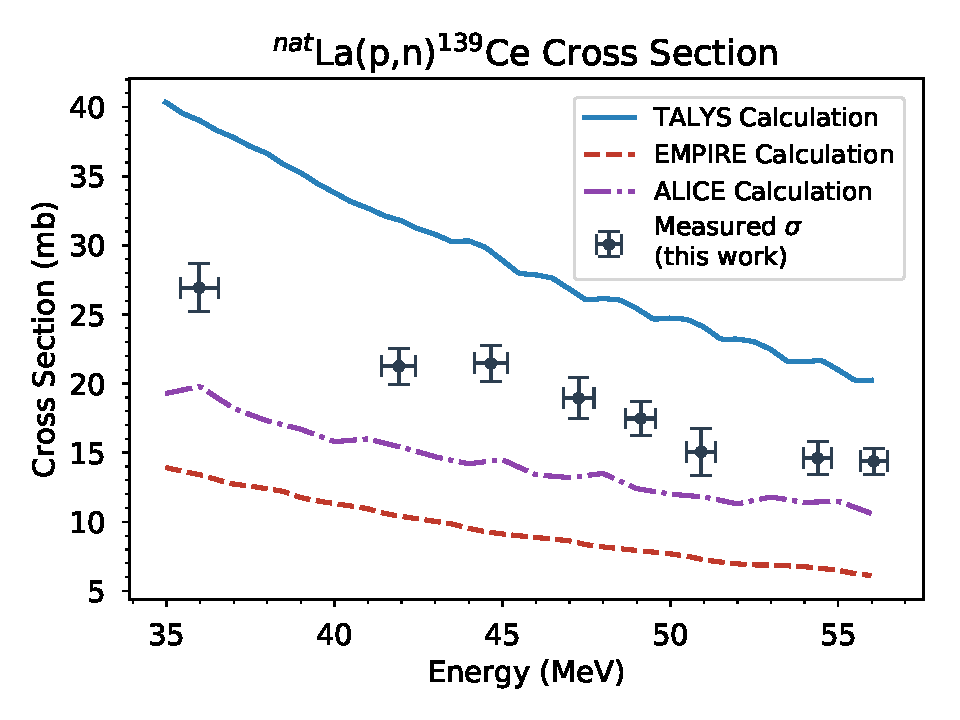
\includegraphics[width=9cm]{cross_sections/139CE}
\caption{Measured cross section for the $^{nat}$La(p,n)$^{139}$Ce reaction, with TALYS (solid blue) and EMPIRE (dashed red) predictions.
}
\label{fig:139CE}
\end{figure}

The measured cross sections for the $^{nat}$La(p,n)$^{139}$Ce reaction are plotted in Fig. \ref{fig:139CE}, along with the TALYS and EMPIRE default outputs.  Both models seem to approximately predict the shape of the cross section, only being off by a constant multiplier.  An adjustment of the level density model could bring these into agreement \cite{BRINK1957215}.

\subsection{$^{nat}$La(p,x)$^{132}$Cs Cross Section}

Despite only producing activities on the order of 1-2 Bq, the $^{nat}$La(p,x)$^{132}$Cs reaction was measureable because its 6.48 day activity was longer than that of most isotopes measured in this study, and because the 97.59 \%, 667.71 keV $\gamma$ line was well isolated and could be counted for multiple days.

\begin{figure}[htb]
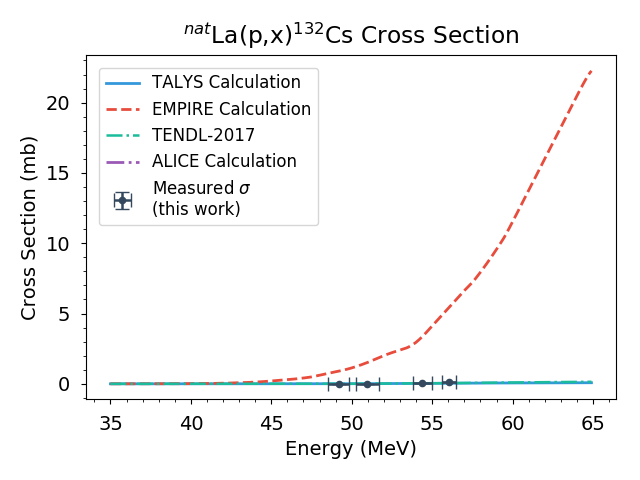
\includegraphics[width=9cm]{cross_sections/132CS}
\caption{Measured cross section for the $^{nat}$La(p,x)$^{132}$Cs reaction, with TALYS (solid blue) and EMPIRE (dashed red) predictions.
}
\label{fig:132CS}
\end{figure}

Fig. \ref{fig:132CS} plots the measured $^{nat}$La(p,x)$^{132}$Cs cross sections, as well as the TALYS and EMPIRE default calculations.  EMPIRE defaults over-predicted this cross section by a factor greater than 20, whereas the TALYS calculation was very close to what was measured.  This discrepancy isn't too surprising as this reaction takes up only a small fraction of the total cross section, and small model adjustments will have a large relative impact on the prediction \cite{KONING2003231}.

\subsection{$^{nat}$La(p,x)$^{133m,133g}$Ba Cross Sections}

Another reaction where the decays of both the isomer and ground state were observed was the $^{nat}$La(p,x)$^{133}$Ba reaction.  The main challenge in this measurement was to identify the $^{133}$Ba ground state decays, which had low activities ($\approx$ 0.1 Bq) due to the 10.55 year half-life of that isotope, and due to contaminating peaks in the spectrum for the first few weeks after the irradiation.  Multiple long counts enabled the identification of the $^{133}$Ba ground state, and separation of the ground state activity due to the population of the isomer.  Fortunately, the isomer has a strong peak (17.69 \%) at 275.92 keV, which allowed its activity to be measured with $<$1\% uncertainty.

\begin{figure}[htb]
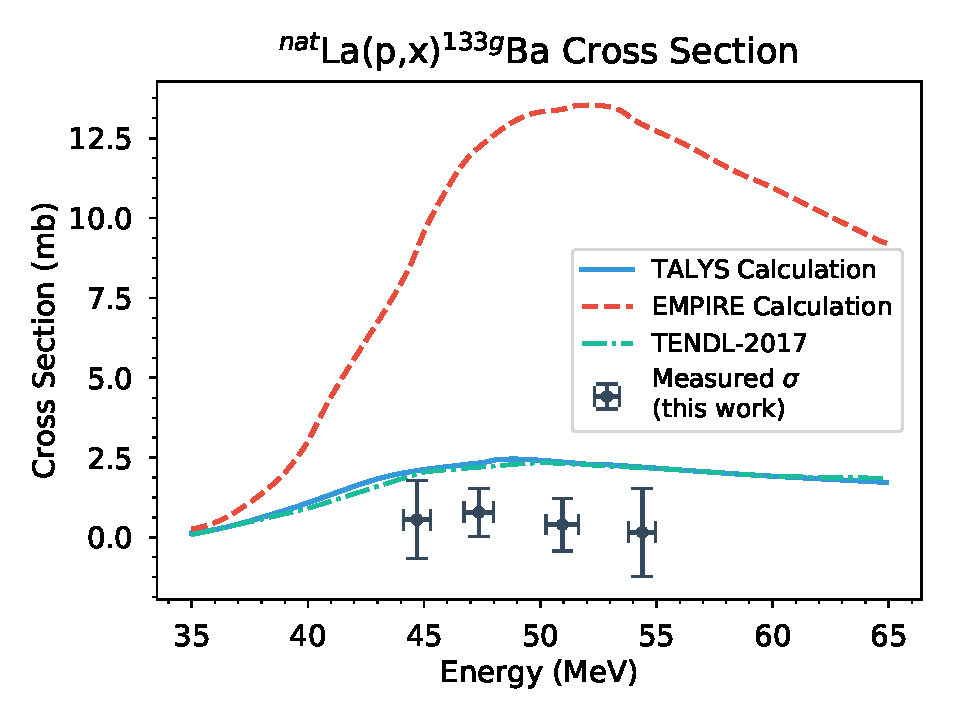
\includegraphics[width=9cm]{cross_sections/133BAg}
\caption{Measured cross section for the $^{nat}$La(p,x)$^{133}$Ba reaction, with TALYS (solid blue) and EMPIRE (dashed red) predictions.
}
\label{fig:133BAg}
\end{figure}

Fig. \ref{fig:133BAg} plots the measured $^{nat}$La(p,x)$^{133g}$Ba reaction cross sections, as well as the TALYS and EMPIRE default calculations.  The relative uncertainties were very large in this channel: the 1$\sigma$ error bars are zero crossing.  However it can be said that this cross section was much smaller than the prediction of either code.

\begin{figure}[htb]
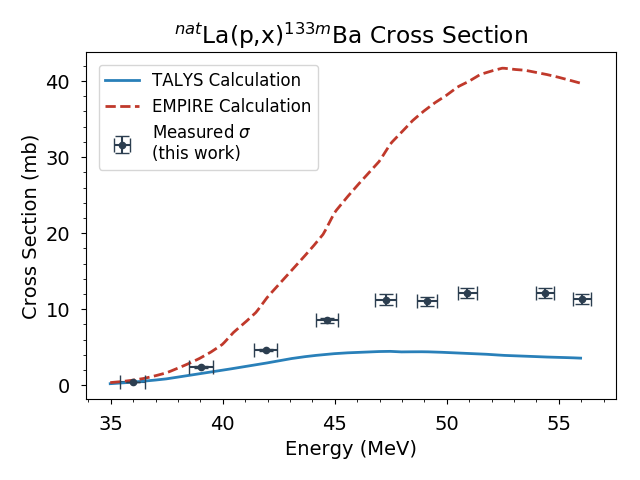
\includegraphics[width=9cm]{cross_sections/133BAm}
\caption{Measured cross section for the $^{nat}$La(p,x)$^{133m}$Ba reaction, with TALYS (solid blue) and EMPIRE (dashed red) predictions.
}
\label{fig:133BAm}
\end{figure}

Fig. \ref{fig:133BAm} plots the measured cross sections for the $^{nat}$La(p,x)$^{133m}$Ba reaction, and TALYS/EMPIRE default calculations.  This measurement was much more precise due to the better counting statistics from the 275.92 keV line.  Here again the EMPIRE code better predicts the energy of the peak of the cross section, however neither code very accurately predicted the magnitude.

\subsection{$^{nat}$La(p,x)$^{135}$La Cross Section}

The final cross section measured in the Lanthanum stack was in the $^{nat}$La(p,x)$^{135}$La reaction, which has relatively weak $\gamma$ emissions but was able to be identified using the 1.52 \%, 480.51 keV $\gamma$ line.  The uncertainties in this measurement were affected by the in-feeding from the decay of $^{135}$Ce, but because the activity of $^{135}$Ce was able to be measured very accurately ($\approx$1\%), this had only a small effect on the uncertainty of the resulting cross section.

\begin{figure}[htb]
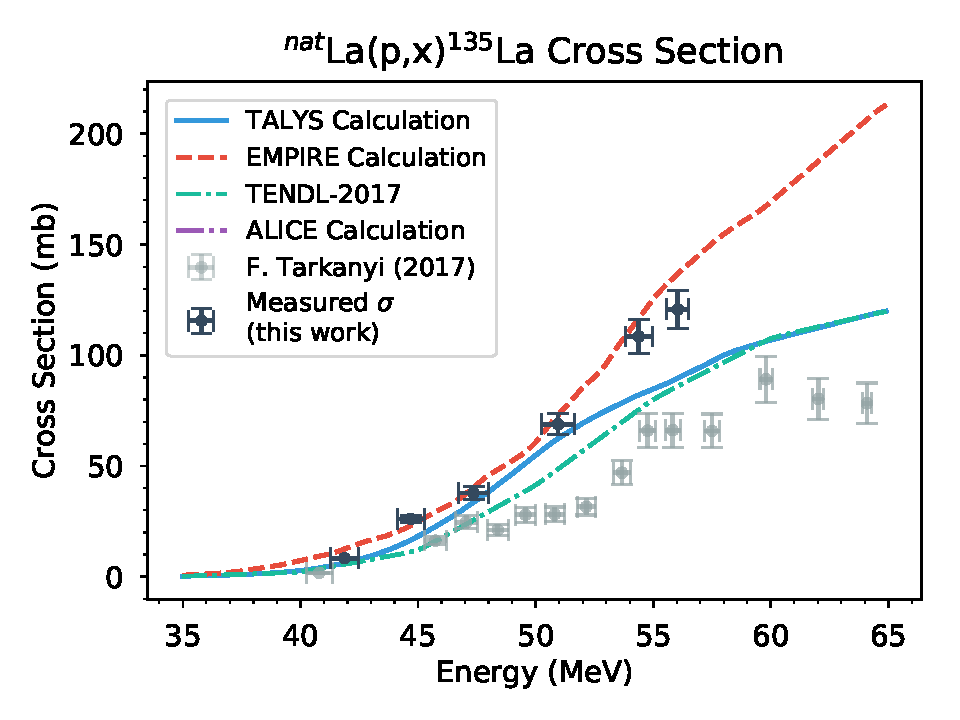
\includegraphics[width=9cm]{cross_sections/135LA}
\caption{Measured cross section for the $^{nat}$La(p,x)$^{135}$La reaction, with TALYS (solid blue) and EMPIRE (dashed red) predictions.
}
\label{fig:135LA}
\end{figure}

Fig. \ref{fig:135LA} plots the measured cross sections for the $^{nat}$La(p,x)$^{135}$La reaction, and TALYS/EMPIRE default calculations.  The EMPIRE model accurately predicts both the shape and magnitude of this cross section, whereas TALYS seems to be predicting the peak of the cross section at lower energy similar to the other reactions.  There are some fluctuations in the EMPIRE predictions, which are likely due to the non-deterministic nature of the pre-equillibrium model it is using \cite{HERMAN20072655}.

\subsection{$^{nat}$Cu(p,x)$^{61}$Cu Cross Section}

The 282.9 keV $\gamma$ line (12.2 \%) from the $^{61}$Cu isotope was observed in the Copper foils used to monitor the proton current, however the $^{nat}$Cu(p,x)$^{61}$Cu reaction isn't currently part of the IAEA charged particle reference (CPR) cross section database \cite{IAEACPR}.  Because the cross sections in this experiment are measured relative to the 2017 CPR evaluation, this measurement may be particularly useful if the $^{nat}$Cu(p,x)$^{61}$Cu reaction is to be added to an upcoming evaluation.

\begin{figure}[htb]
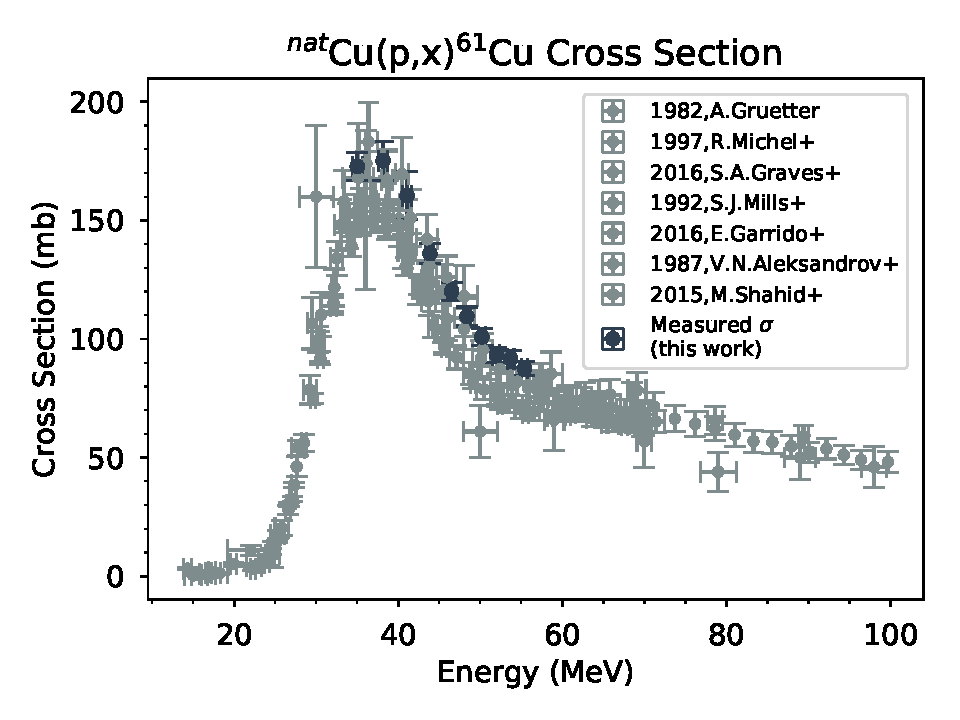
\includegraphics[width=9cm]{cross_sections/61CU}
\caption{Measured cross section for the $^{nat}$Cu(p,x)$^{61}$Cu reaction, with other measurements from the EXFOR database.
}
\label{fig:61CU}
\end{figure}

The measured cross sections for the $^{nat}$Cu(p,x)$^{61}$Cu reaction are plotted in Fig. \ref{fig:61CU}, along with measurements done in previous experiments that have submitted entries into the EXFOR database.  There is clear agreement with the measurements from EXFOR, both in the shape and magnitude of the cross sections measured in this experiment.  This provides confidence in the proton current measured by the monitor foils, the energy assignments as determined by the minimization technique, as well as the overall measurement and data reduction methodology.


\section{Summary and Conclusions}
In this experiment we measured the cross sections for various $^{nat}$La(p,x) reactions using a 57 MeV proton beam at the LBNL 88" cyclotron and a stacked foil target.  We also compared these measurements with the outputs of the TALYS and EMPIRE nuclear reaction modelling codes, using default parameters.  In most cases neither code accurately predicted the magnitude of the cross sections, but TALYS consistently underpredicted the energy of the peak in the cross section, whereas the EMPIRE predictions agreed with the shape of the measured cross sections quite well.  This primarily speaks to the fidelity of the pre-equillibrium models used by the respective codes: the hybrid Monte Carlo simulation model typically produced better predictions than the exiton model.

Particular emphasis was placed on the production of $^{134}$Ce, an isotope with applications as a positron emitting analogue of the medically relevant $^{225}$Ac isotope.  The results of this study show that in order to produce significant quantities of $^{134}$Ce from the $^{nat}$La(p,6n) reaction a higher energy proton beam is required.  The highest energy proton beam availible at the LBNL 88" cyclotron (57 MeV) produces an unacceptable activity of other Cerium isotopes, which will act as impurities in a medical study.  A proton beam of at least 70 MeV will be required to produce significant activities of $^{134}$Ce without contaminants.

\section*{Acknowledgements}
We wish to acknowledge our thanks to the operators of the 88" cyclotron: Brien Ninemire, Nick Brickner, Tom Gimpel and Scott Small for their efforts in setting a new "high-water mark" for the maximum proton energy extracted from the machine.  This work has been performed under the auspices of the U.S. Department of Energy by Lawrence Berkeley National Laboratory under contract No. LAB16-1588 NSD.
\bibliography{LaCe}

\appendix
\section{Table of Cross Sections}
\label{xs_appendix}
\ \ 
\begin{ruledtabular}
\begin{tabular}{ccc}
Isotope & E [MeV] & $\sigma$ [mb] \\

\hline
\multicolumn{3}{l}{\textit{Independent}} \\ 
$^{134}$Ce & 56.06 $\pm$ 0.4 & 33.772 $\pm$ 2.171 \\ 
$^{134}$Ce & 54.39 $\pm$ 0.41 & 11.269 $\pm$ 0.712 \\ 
$^{134}$Ce & 50.92 $\pm$ 0.44 & 2.113 $\pm$ 0.148 \\ 
$^{134}$Ce & 49.12 $\pm$ 0.45 & 0.929 $\pm$ 0.057 \\ 
\hline
\multicolumn{3}{l}{\textit{Cumulative}} \\ 
$^{135}$Ce & 56.06 $\pm$ 0.4 & 418.262 $\pm$ 25.258 \\ 
$^{135}$Ce & 54.39 $\pm$ 0.41 & 429.893 $\pm$ 25.191 \\ 
$^{135}$Ce & 50.92 $\pm$ 0.44 & 342.967 $\pm$ 19.485 \\ 
$^{135}$Ce & 49.12 $\pm$ 0.45 & 303.12 $\pm$ 16.909 \\ 
$^{135}$Ce & 47.27 $\pm$ 0.46 & 231.253 $\pm$ 16.929 \\ 
$^{135}$Ce & 44.66 $\pm$ 0.48 & 108.902 $\pm$ 4.479 \\ 
$^{135}$Ce & 41.92 $\pm$ 0.51 & 26.697 $\pm$ 1.074 \\ 
$^{135}$Ce & 39.04 $\pm$ 0.53 & 2.634 $\pm$ 0.144 \\ 
$^{135}$Ce & 35.98 $\pm$ 0.57 & 0.451 $\pm$ 0.022 \\ 
\hline
\multicolumn{3}{l}{\textit{Independent}} \\ 
$^{137m}$Ce & 56.06 $\pm$ 0.4 & 81.102 $\pm$ 4.769 \\ 
$^{137m}$Ce & 54.39 $\pm$ 0.41 & 89.677 $\pm$ 5.159 \\ 
$^{137m}$Ce & 50.92 $\pm$ 0.44 & 97.182 $\pm$ 5.337 \\ 
$^{137m}$Ce & 49.12 $\pm$ 0.45 & 111.87 $\pm$ 6.025 \\ 
$^{137m}$Ce & 47.27 $\pm$ 0.46 & 125.648 $\pm$ 7.969 \\ 
$^{137m}$Ce & 44.66 $\pm$ 0.48 & 149.717 $\pm$ 5.759 \\ 
$^{137m}$Ce & 41.92 $\pm$ 0.51 & 178.751 $\pm$ 6.709 \\ 
$^{137m}$Ce & 39.04 $\pm$ 0.53 & 317.464 $\pm$ 16.817 \\ 
$^{137m}$Ce & 35.98 $\pm$ 0.57 & 448.639 $\pm$ 17.976 \\ 
\hline
\multicolumn{3}{l}{\textit{Independent}} \\ 
$^{137g}$Ce & 56.06 $\pm$ 0.4 & 24.724 $\pm$ 1.841 \\ 
$^{137g}$Ce & 54.39 $\pm$ 0.41 & 28.222 $\pm$ 2.073 \\ 
$^{137g}$Ce & 50.92 $\pm$ 0.44 & 27.944 $\pm$ 1.997 \\ 
$^{137g}$Ce & 49.12 $\pm$ 0.45 & 27.367 $\pm$ 1.933 \\ 
$^{137g}$Ce & 47.27 $\pm$ 0.46 & 34.033 $\pm$ 2.66 \\ 
$^{137g}$Ce & 44.66 $\pm$ 0.48 & 38.399 $\pm$ 2.294 \\ 
$^{137g}$Ce & 41.92 $\pm$ 0.51 & 39.374 $\pm$ 2.328 \\ 
$^{137g}$Ce & 39.04 $\pm$ 0.53 & 59.264 $\pm$ 4.146 \\ 
$^{137g}$Ce & 35.98 $\pm$ 0.57 & 80.142 $\pm$ 4.87 \\ 
\hline
\multicolumn{3}{l}{\textit{Cumulative}} \\ 
$^{139}$Ce & 56.06 $\pm$ 0.4 & 14.374 $\pm$ 0.938 \\ 
$^{139}$Ce & 54.39 $\pm$ 0.41 & 14.602 $\pm$ 1.191 \\ 
$^{139}$Ce & 50.92 $\pm$ 0.44 & 15.064 $\pm$ 1.698 \\ 
$^{139}$Ce & 49.12 $\pm$ 0.45 & 17.472 $\pm$ 1.239 \\ 
$^{139}$Ce & 47.27 $\pm$ 0.46 & 18.932 $\pm$ 1.483 \\ 
$^{139}$Ce & 44.66 $\pm$ 0.48 & 21.465 $\pm$ 1.305 \\ 
$^{139}$Ce & 41.92 $\pm$ 0.51 & 21.255 $\pm$ 1.311 \\ 
$^{139}$Ce & 35.98 $\pm$ 0.57 & 26.94 $\pm$ 1.722 \\ 
\hline
\multicolumn{3}{l}{\textit{Independent}} \\ 
$^{132}$Cs & 56.06 $\pm$ 0.4 & 0.107 $\pm$ 0.006 \\ 
$^{132}$Cs & 54.39 $\pm$ 0.41 & 0.073 $\pm$ 0.004 \\ 
$^{132}$Cs & 50.92 $\pm$ 0.44 & 0.017 $\pm$ 0.001 \\ 
$^{132}$Cs & 49.12 $\pm$ 0.45 & 0.013 $\pm$ 0.001 \\ 
\hline
\multicolumn{3}{l}{\textit{Independent}} \\ 
$^{133m}$Ba & 56.06 $\pm$ 0.4 & 11.364 $\pm$ 0.659 \\ 
$^{133m}$Ba & 54.39 $\pm$ 0.41 & 12.157 $\pm$ 0.683 \\ 
$^{133m}$Ba & 50.92 $\pm$ 0.44 & 12.171 $\pm$ 0.661 \\ 
$^{133m}$Ba & 49.12 $\pm$ 0.45 & 11.056 $\pm$ 0.588 \\ 
$^{133m}$Ba & 47.27 $\pm$ 0.46 & 11.236 $\pm$ 0.706 \\ 
$^{133m}$Ba & 44.66 $\pm$ 0.48 & 8.552 $\pm$ 0.321 \\ 
$^{133m}$Ba & 41.92 $\pm$ 0.51 & 4.65 $\pm$ 0.17 \\ 
$^{133m}$Ba & 39.04 $\pm$ 0.53 & 2.379 $\pm$ 0.142 \\ 
$^{133m}$Ba & 35.98 $\pm$ 0.57 & 0.461 $\pm$ 0.024 \\ 
\hline
\multicolumn{3}{l}{\textit{Independent}} \\ 
$^{133g}$Ba & 54.39 $\pm$ 0.41 & 0.16 $\pm$ 1.379 \\ 
$^{133g}$Ba & 50.92 $\pm$ 0.44 & 0.403 $\pm$ 0.831 \\ 
$^{133g}$Ba & 47.27 $\pm$ 0.46 & 0.789 $\pm$ 0.752 \\ 
$^{133g}$Ba & 44.66 $\pm$ 0.48 & 0.556 $\pm$ 1.23 \\ 
\hline
\multicolumn{3}{l}{\textit{Independent}} \\ 
$^{135}$La & 56.06 $\pm$ 0.4 & 121.127 $\pm$ 8.522 \\ 
$^{135}$La & 54.39 $\pm$ 0.41 & 108.826 $\pm$ 7.504 \\ 
$^{135}$La & 50.92 $\pm$ 0.44 & 69.106 $\pm$ 4.648 \\ 
$^{135}$La & 47.27 $\pm$ 0.46 & 37.889 $\pm$ 3.095 \\ 
$^{135}$La & 44.66 $\pm$ 0.48 & 26.209 $\pm$ 1.435 \\ 
$^{135}$La & 41.92 $\pm$ 0.51 & 8.432 $\pm$ 0.483 \\ 
\hline
\multicolumn{3}{l}{\textit{Independent}} \\ 
$^{61}$Cu & 55.38 $\pm$ 0.41 & 87.538 $\pm$ 2.982 \\ 
$^{61}$Cu & 53.69 $\pm$ 0.42 & 91.609 $\pm$ 3.531 \\ 
$^{61}$Cu & 51.96 $\pm$ 0.43 & 93.288 $\pm$ 3.037 \\ 
$^{61}$Cu & 50.19 $\pm$ 0.44 & 100.853 $\pm$ 3.724 \\ 
$^{61}$Cu & 48.36 $\pm$ 0.45 & 109.481 $\pm$ 4.003 \\ 
$^{61}$Cu & 46.49 $\pm$ 0.47 & 120.098 $\pm$ 3.779 \\ 
$^{61}$Cu & 43.85 $\pm$ 0.49 & 135.949 $\pm$ 4.298 \\ 
$^{61}$Cu & 41.06 $\pm$ 0.51 & 160.339 $\pm$ 10.096 \\ 
$^{61}$Cu & 38.14 $\pm$ 0.54 & 175.09 $\pm$ 8.116 \\ 
$^{61}$Cu & 35.0 $\pm$ 0.58 & 172.693 $\pm$ 6.006 \\ \end{tabular}
\label{table:all_xs}
\end{ruledtabular}
\ \ 

\section{Stack Design}
\label{stack_appendix}
\ \ 
\begin{ruledtabular}
\begin{tabular}{cccc}
Foil Id & Compound & $\Delta x$ [mm] & $\rho \Delta x$ [mg/cm$^2$] \\
SS3 & 316 SS & 0.13 & 100.48 $\pm$ 0.46 \\
La01 & La & 0.0275 & 14.59 $\pm$ 0.69 \\
Al01 & Al & 0.027 & 6.58 $\pm$ 0.02 \\
Cu01 & Cu & 0.029 & 22.13 $\pm$ 0.07 \\
E1 & Al & 0.254 & 68.53 $\pm$ 5.08 \\
La02 & La & 0.0278 & 15.55 $\pm$ 0.71 \\
Al02 & Al & 0.0278 & 6.67 $\pm$ 0.12 \\
Cu02 & Cu & 0.0293 & 22.23 $\pm$ 0.44 \\
E2 & Al & 0.254 & 68.53 $\pm$ 5.08 \\
La03 & La & 0.0315 & 15.12 $\pm$ 0.83 \\
Al03 & Al & 0.027 & 6.7 $\pm$ 0.03 \\
Cu03 & Cu & 0.031 & 22.24 $\pm$ 0.07 \\
E3 & Al & 0.254 & 68.53 $\pm$ 5.08 \\
La04 & La & 0.0288 & 14.95 $\pm$ 0.66 \\
Al04 & Al & 0.027 & 6.68 $\pm$ 0.03 \\
Cu04 & Cu & 0.0317 & 22.49 $\pm$ 0.42 \\
E4 & Al & 0.254 & 68.53 $\pm$ 5.08 \\
La05 & La & 0.027 & 15.07 $\pm$ 0.65 \\
Al05 & Al & 0.027 & 6.64 $\pm$ 0.01 \\
Cu05 & Cu & 0.0313 & 22.39 $\pm$ 0.42 \\
E5 & Al & 0.254 & 68.53 $\pm$ 5.08 \\
La06 & La & 0.026 & 14.32 $\pm$ 0.78 \\
Al06 & Al & 0.0278 & 6.66 $\pm$ 0.23 \\
Cu06 & Cu & 0.031 & 22.22 $\pm$ 0.05 \\
E6+E7 & Al & 0.508 & 137.06 $\pm$ 10.16 \\
La07 & La & 0.0258 & 14.21 $\pm$ 0.29 \\
Al07 & Al & 0.0273 & 6.64 $\pm$ 0.12 \\
Cu07 & Cu & 0.031 & 22.4 $\pm$ 0.05 \\
E8+E9 & Al & 0.508 & 137.06 $\pm$ 10.16 \\
La08 & La & 0.0283 & 15.64 $\pm$ 0.28 \\
Al08 & Al & 0.0273 & 6.72 $\pm$ 0.13 \\
Cu08 & Cu & 0.032 & 22.16 $\pm$ 1.2 \\
E10+E11 & Al & 0.508 & 137.06 $\pm$ 10.16 \\
La09 & La & 0.0268 & 12.67 $\pm$ 0.51 \\
Al09 & Al & 0.0275 & 6.65 $\pm$ 0.14 \\
Cu09 & Cu & 0.031 & 22.2 $\pm$ 0.72 \\
E12+E13 & Al & 0.508 & 137.06 $\pm$ 10.16 \\
La10 & La & 0.0278 & 16.14 $\pm$ 0.3 \\
Al10 & Al & 0.027 & 6.73 $\pm$ 0.02 \\
Cu10 & Cu & 0.031 & 22.5 $\pm$ 0.05 \\
SS4 & 316 SS & 0.13 & 101.26 $\pm$ 0.79 \\\end{tabular}
\label{table:stack}
\end{ruledtabular}
\ \ 



\section{Relevant Nuclear Data \cite{ensdf}}
\label{nudat_appendix}
\ \ 
\begin{ruledtabular}
\begin{tabular}{cccc}
Isotope & $\gamma$ Energy (keV) & $I_{\gamma}$ (\%) & $T_{1/2}$ \\
$^{134}$Ce & - & - & 3.16 (4) d \\
$^{134}$La & 604.721 & 5.04 (20) & 6.45 (16) s \\
$^{135}$Ce & 265.56 & 41.8 (14) & 17.7 (3) h \\
$^{137m}$Ce & 254.29 & 11.1 (4) & 34.4 (3) h \\
$^{137g}$Ce & 447.15 & 1.68 (?) & 9.0 (3) h \\
$^{139g}$Ce & 165.85 & 80.0 (?) & 137.64 (2) d \\
$^{135}$La & 480.51 & 1.52 (?) & 19.5 (2) h \\
$^{133m}$Ba & 275.925 & 17.69 (?) & 38.93 (1) h \\
$^{133g}$Ba & 356.013 & 62.05 (?) & 10.551 (11) y \\
$^{132}$Cs & 667.714 & 97.59 (?) & 6.480 (6) d \\
$^{61}$Cu & 282.956 & 12.2 (?) & 3.339 (8) h \\
$^{62}$Zn & 596.56 & 26.0 (?) & 9.193 (15) h \\
$^{63}$Zn & 669.62 & 8.2 (?) & 38.47 (5) m \\
$^{58}$Co & 810.759 & 99.45 (?) & 70.86 (6) d \\
$^{22}$Na & 1274.537 & 99.940 (14) & 2.6018 (22) y \\
$^{24}$Na & 1368.626 & 99.9936 (15) & 14.997 (12) h \\
\end{tabular}
\label{table:stack}
\end{ruledtabular}
\ \ 


\end{document}